% ========================================
% Diagrama 7D: Estrutura de Diretórios (TikZ/LaTeX)
% Formato: TikZ - Pronto para usar em papers LaTeX
% Como usar: % ========================================
% Diagrama 7D: Estrutura de Diretórios (TikZ/LaTeX)
% Formato: TikZ - Pronto para usar em papers LaTeX
% Como usar: % ========================================
% Diagrama 7D: Estrutura de Diretórios (TikZ/LaTeX)
% Formato: TikZ - Pronto para usar em papers LaTeX
% Como usar: % ========================================
% Diagrama 7D: Estrutura de Diretórios (TikZ/LaTeX)
% Formato: TikZ - Pronto para usar em papers LaTeX
% Como usar: \input{07_directory_structure.tex} ou compilar standalone
% ========================================

\documentclass[tikz,border=10pt]{standalone}
\usepackage{tikz}
\usetikzlibrary{trees,positioning,arrows.meta,shapes.geometric,calc}
\usepackage{fontawesome5} % Para ícones (opcional)

\begin{document}

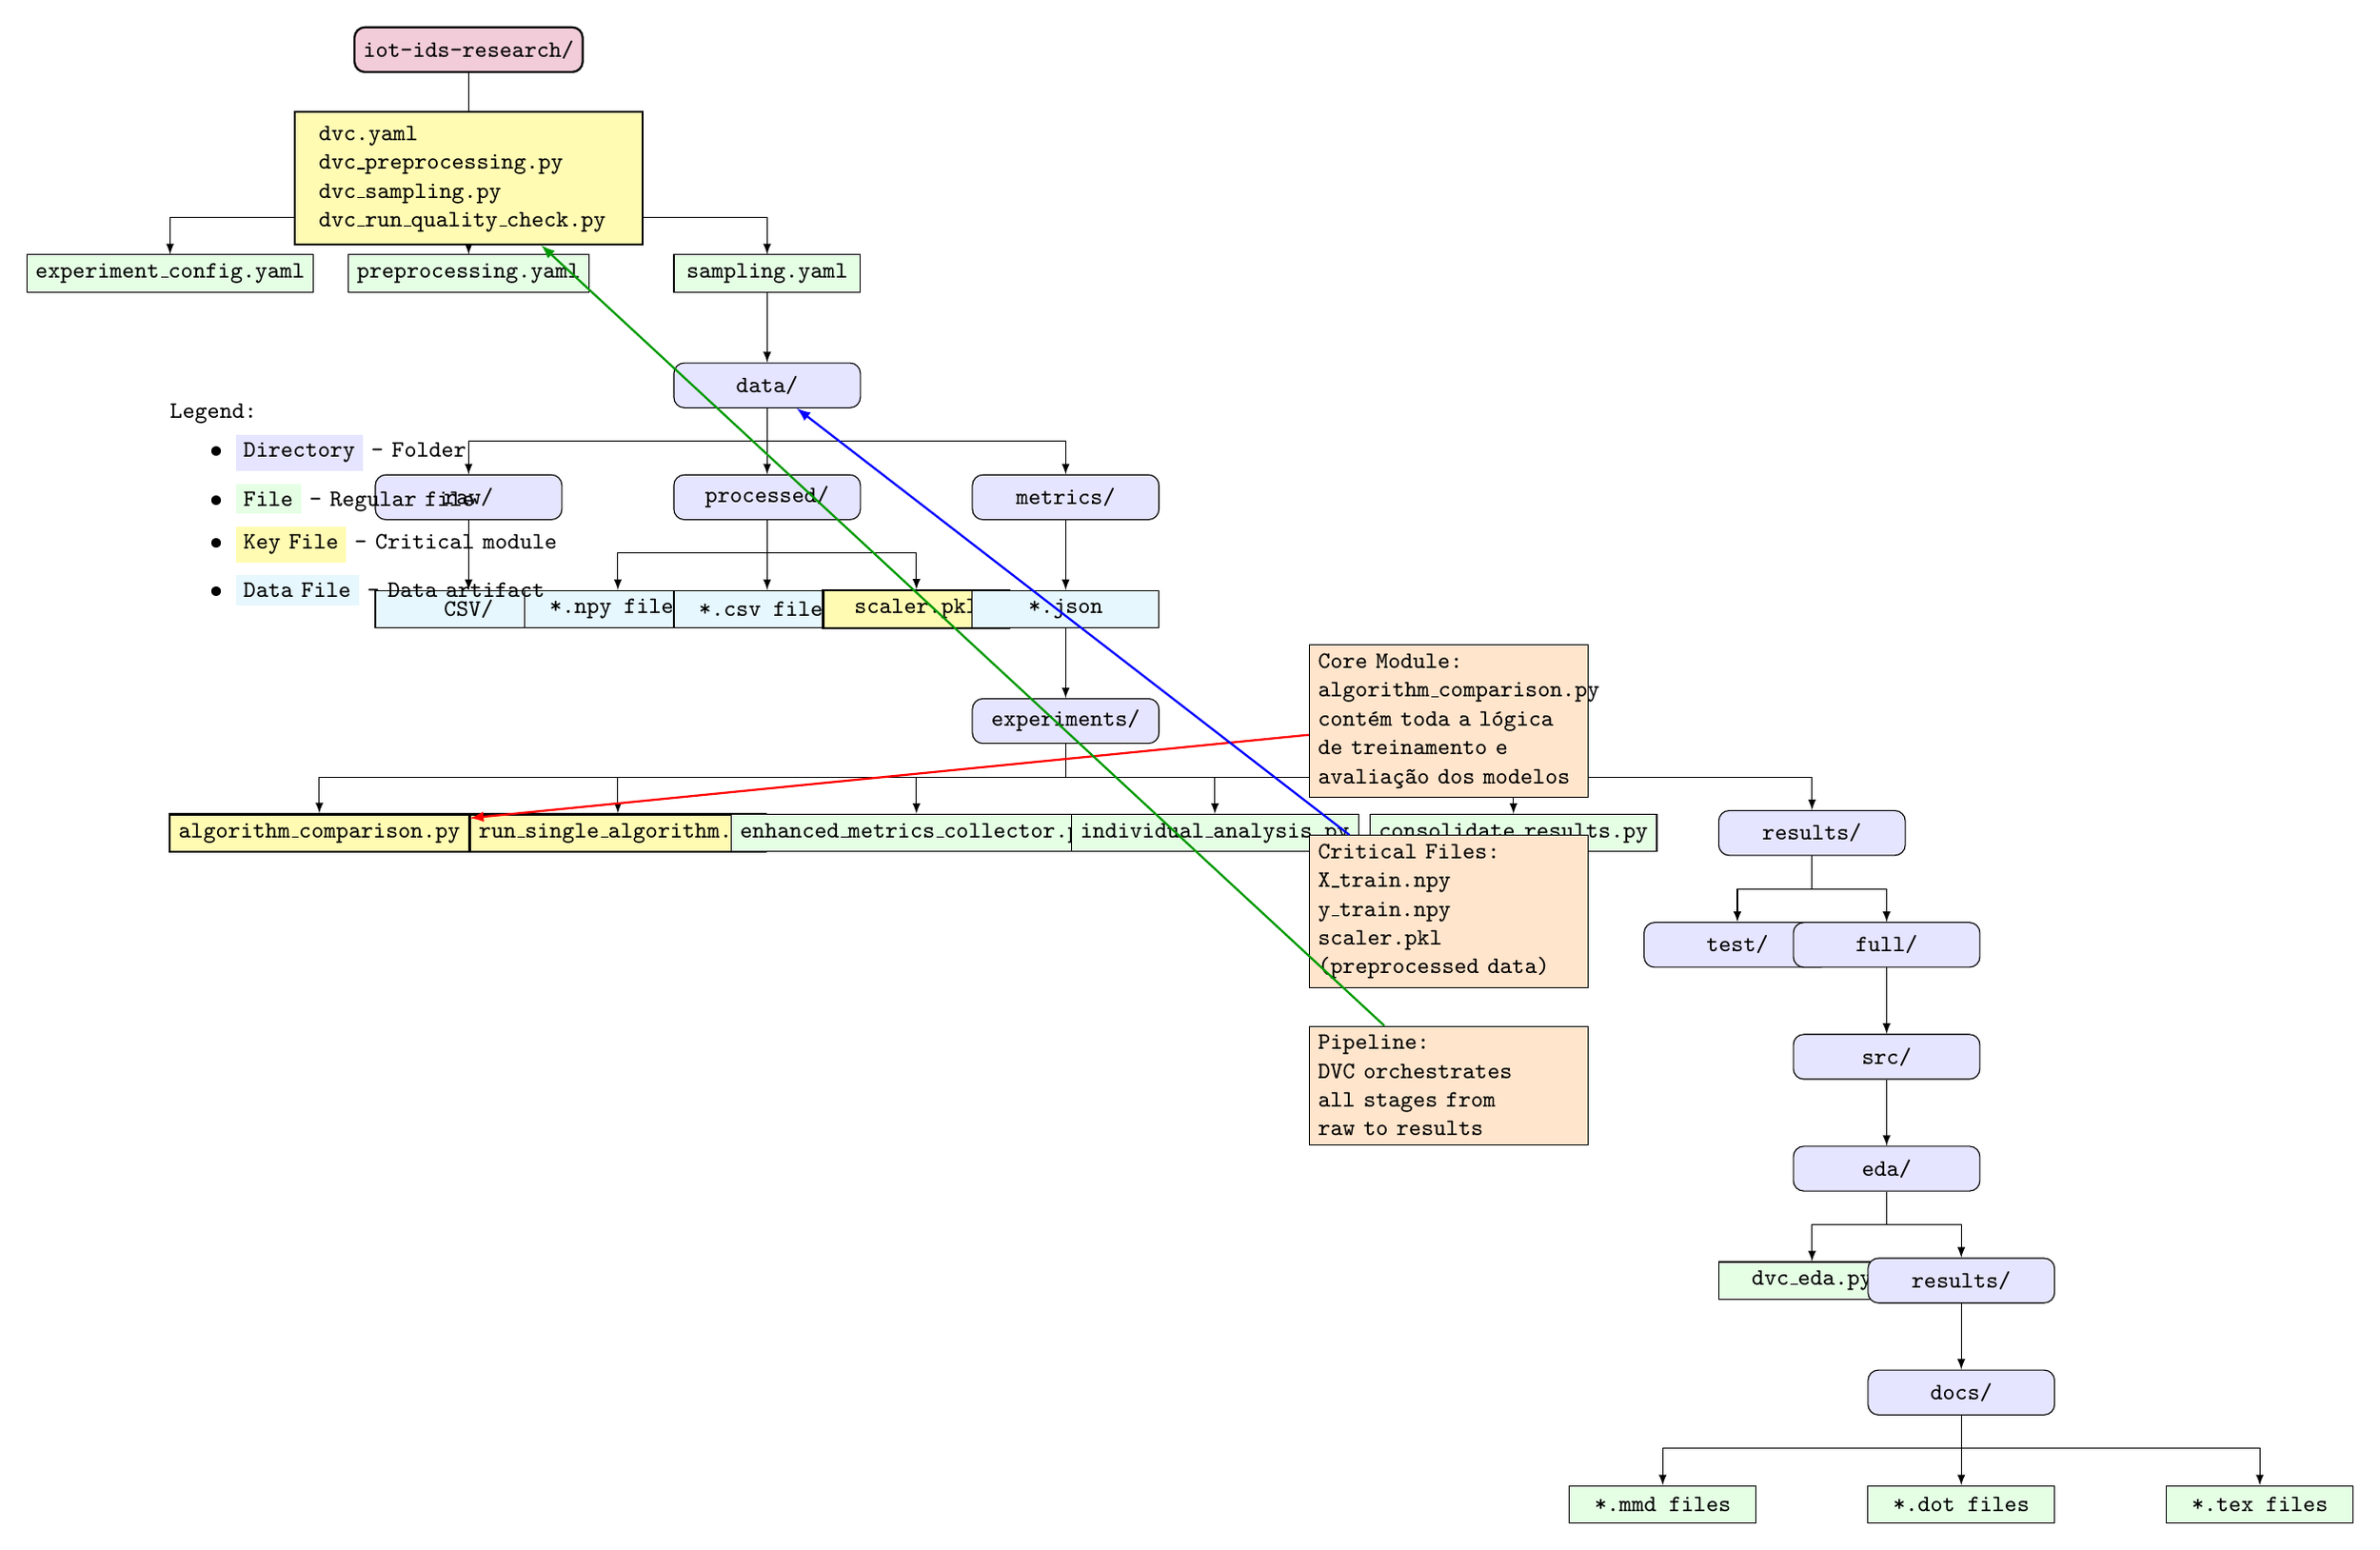
\begin{tikzpicture}[
    % Estilos dos nós
    every node/.style={font=\small\ttfamily},
    dir/.style={draw, rectangle, rounded corners, fill=blue!10, 
                minimum width=2.5cm, minimum height=0.6cm, align=left},
    file/.style={draw, rectangle, fill=green!10, 
                 minimum width=2.5cm, minimum height=0.5cm, align=left},
    key_file/.style={draw, rectangle, fill=yellow!30, 
                     minimum width=2.5cm, minimum height=0.5cm, align=left, thick},
    data_file/.style={draw, rectangle, fill=cyan!10,
                      minimum width=2.5cm, minimum height=0.5cm, align=left},
    level 1/.style={sibling distance=8cm, level distance=1.5cm},
    level 2/.style={sibling distance=4cm, level distance=1.5cm},
    level 3/.style={sibling distance=2cm, level distance=1.5cm},
    edge from parent/.style={draw, -latex}
]

% Root
\node[dir, fill=purple!20, thick] (root) {iot-ids-research/}
    [edge from parent fork down]
    
    % Nível 1 - Principais diretórios
    child { node[dir] (configs) {configs/}
        child { node[file] {experiment\_config.yaml} }
        child { node[file] {preprocessing.yaml} }
        child { node[file] {sampling.yaml} }
    }
    
    child { node[dir] (data) {data/}
        child { node[dir] {raw/}
            child { node[data_file] {CSV/} }
        }
        child { node[dir] {processed/}
            child { node[data_file] {*.npy files} }
            child { node[data_file] {*.csv files} }
            child { node[key_file] {scaler.pkl} }
        }
        child { node[dir] {metrics/}
            child { node[data_file] {*.json} }
        }
    }
    
    child { node[dir] (experiments) {experiments/}
        child { node[key_file] (algo_comp) {algorithm\_comparison.py} }
        child { node[key_file] {run\_single\_algorithm.py} }
        child { node[file] {enhanced\_metrics\_collector.py} }
        child { node[file] {individual\_analysis.py} }
        child { node[file] {consolidate\_results.py} }
        child { node[dir] {results/}
            child { node[dir] {test/} }
            child { node[dir] {full/} }
        }
    }
    
    child { node[dir] (src) {src/}
        child { node[dir] {eda/}
            child { node[file] {dvc\_eda.py} }
            child { node[dir] {results/} }
        }
    }
    
    child { node[dir] (docs) {docs/}
        child { node[file] {*.mmd files} }
        child { node[file] {*.dot files} }
        child { node[file] {*.tex files} }
    };

% DVC scripts no root
\node[key_file, below=0.5cm of root] (dvc_scripts) {
    \begin{tabular}{l}
    dvc.yaml \\
    dvc\_preprocessing.py \\
    dvc\_sampling.py \\
    dvc\_run\_quality\_check.py
    \end{tabular}
};

% Anotações e setas explicativas
\node[draw, rectangle, fill=orange!20, text width=3.5cm, align=left, right=2cm of experiments] (note1) {
    \textbf{Core Module:}\\
    algorithm\_comparison.py\\
    contém toda a lógica\\
    de treinamento e\\
    avaliação dos modelos
};

\draw[-latex, thick, red] (note1) -- (algo_comp);

\node[draw, rectangle, fill=orange!20, text width=3.5cm, align=left, below=0.5cm of note1] (note2) {
    \textbf{Critical Files:}\\
    X\_train.npy\\
    y\_train.npy\\
    scaler.pkl\\
    (preprocessed data)
};

\draw[-latex, thick, blue] (note2) -- (data);

\node[draw, rectangle, fill=orange!20, text width=3.5cm, align=left, below=0.5cm of note2] (note3) {
    \textbf{Pipeline:}\\
    DVC orchestrates\\
    all stages from\\
    raw to results
};

\draw[-latex, thick, green!60!black] (note3) -- (dvc_scripts);

% Legenda
\node[below=2cm of dvc_scripts, text width=8cm, align=left] (legend) {
    \textbf{Legend:}
    \begin{itemize}
        \item \colorbox{blue!10}{Directory} - Folder
        \item \colorbox{green!10}{File} - Regular file
        \item \colorbox{yellow!30}{\textbf{Key File}} - Critical module
        \item \colorbox{cyan!10}{Data File} - Data artifact
    \end{itemize}
};

\end{tikzpicture}

\end{document}

 ou compilar standalone
% ========================================

\documentclass[tikz,border=10pt]{standalone}
\usepackage{tikz}
\usetikzlibrary{trees,positioning,arrows.meta,shapes.geometric,calc}
\usepackage{fontawesome5} % Para ícones (opcional)

\begin{document}

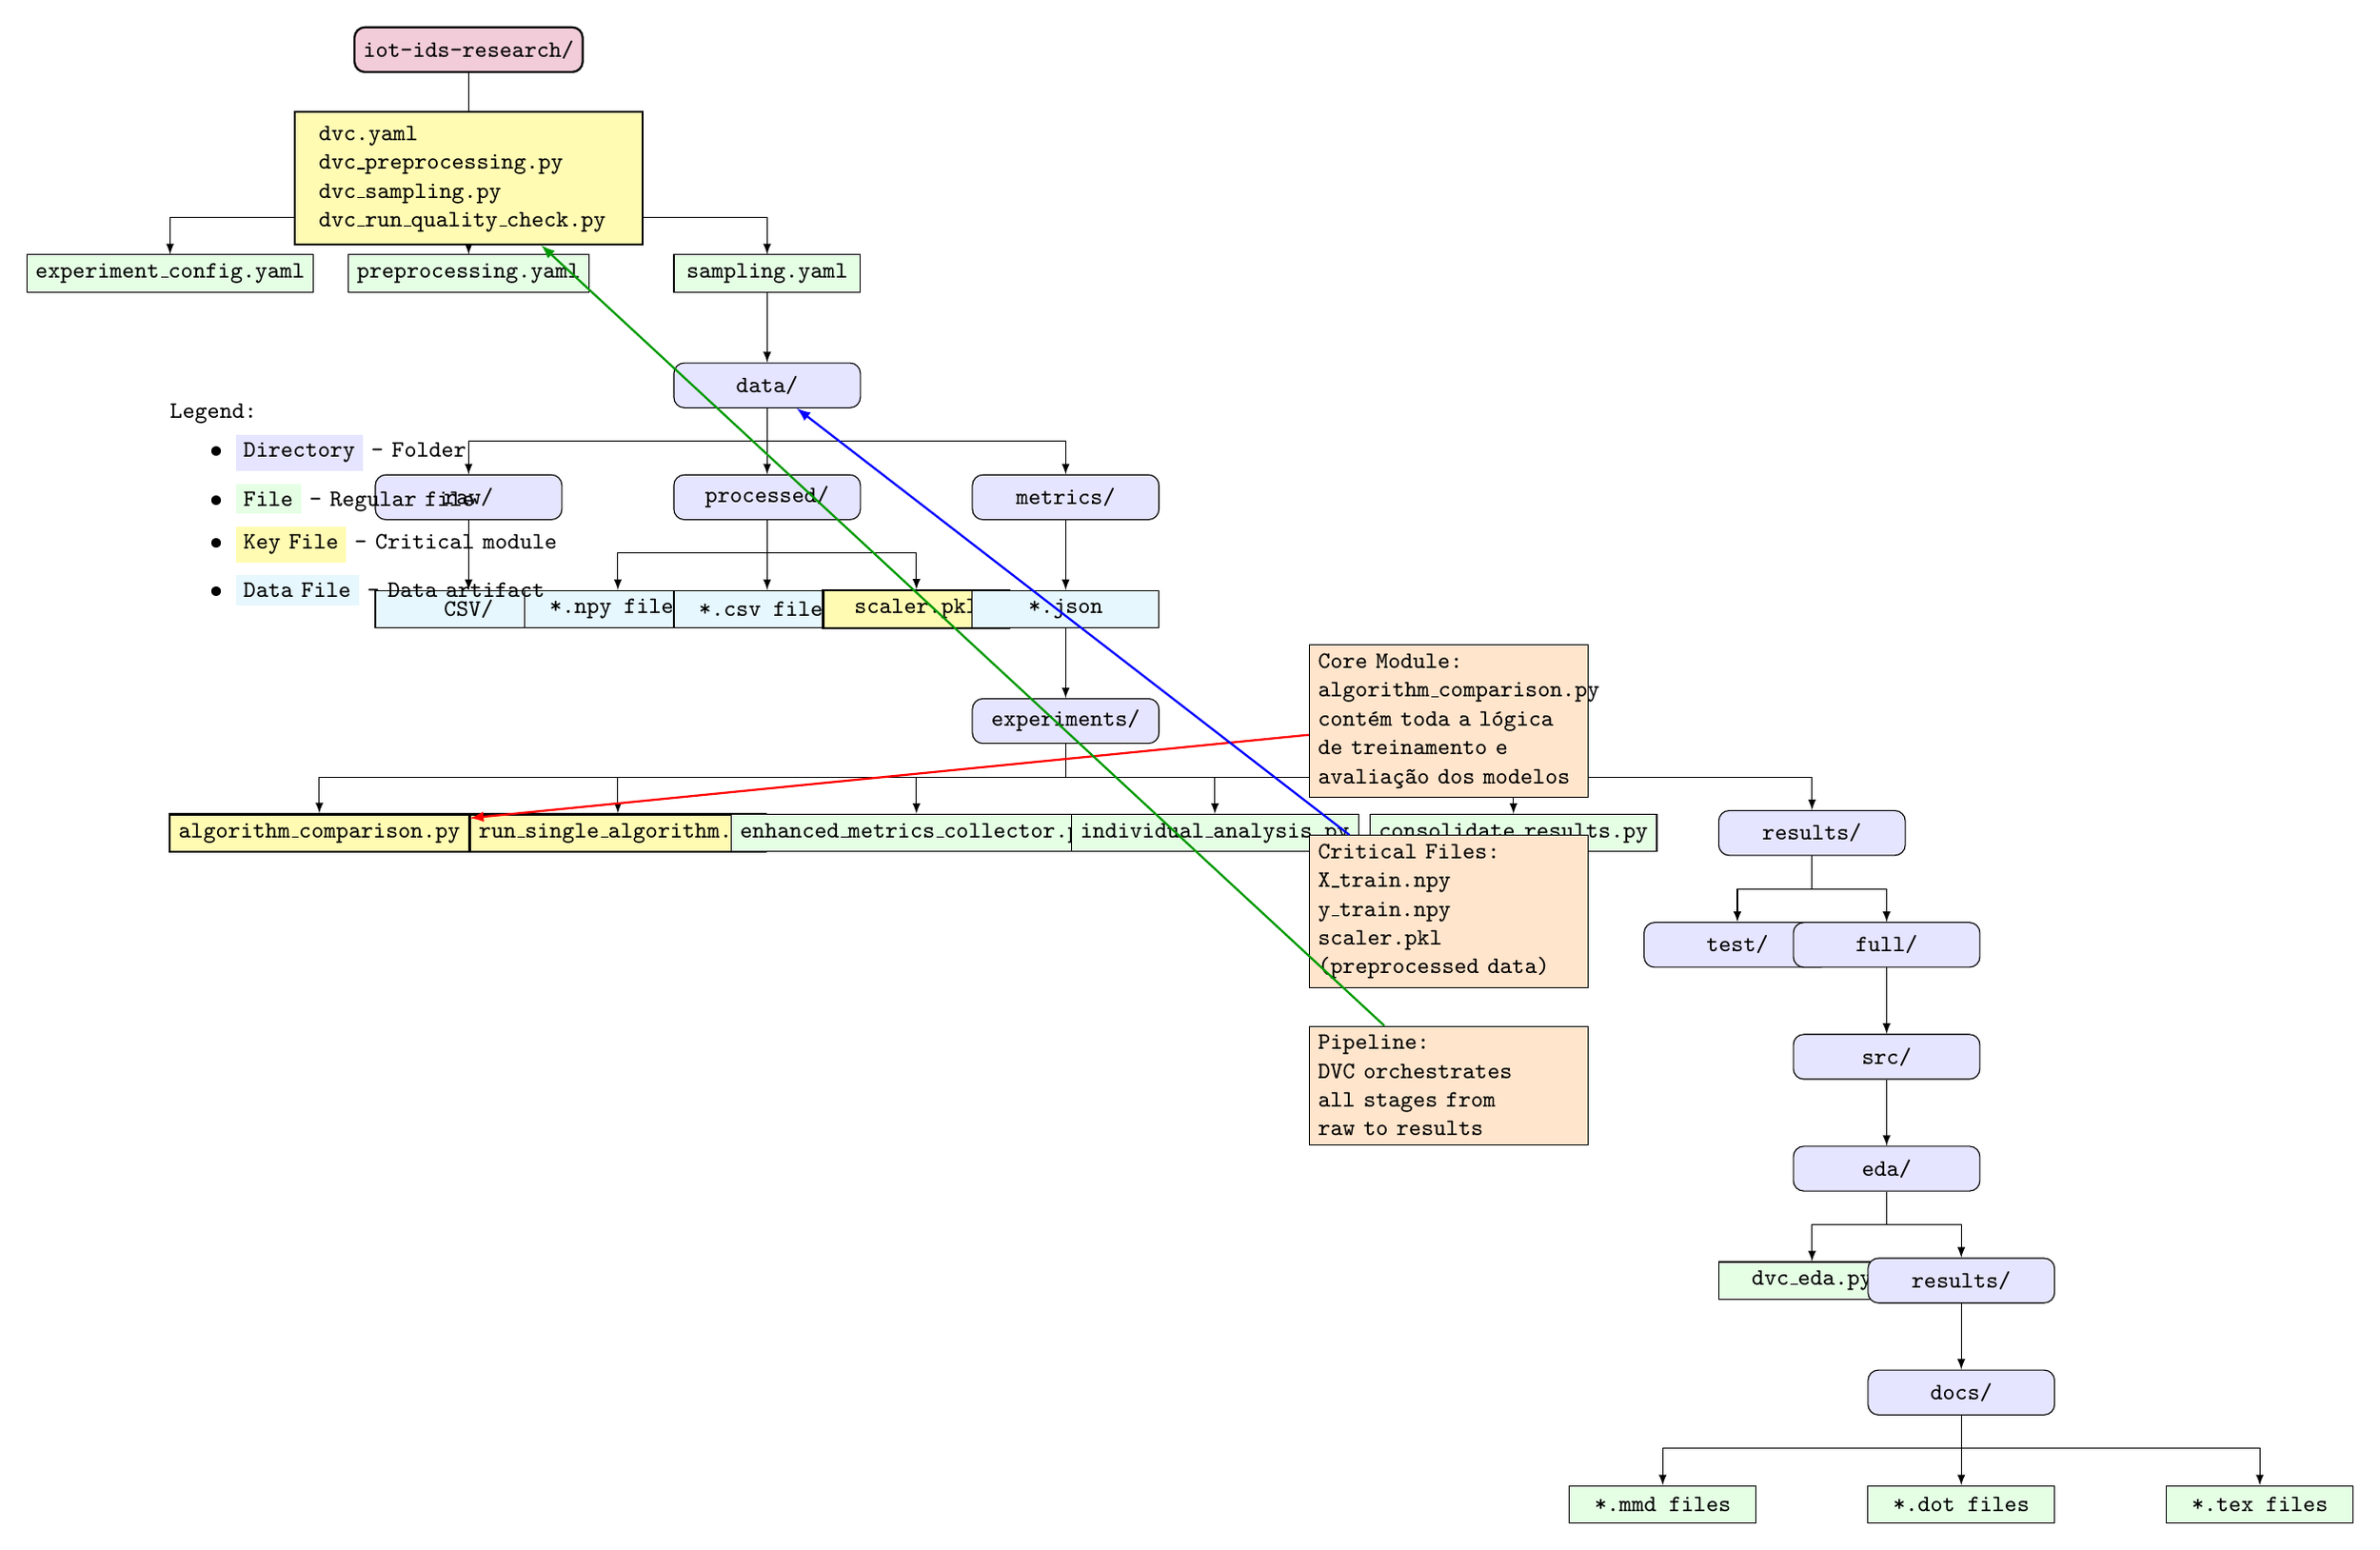
\begin{tikzpicture}[
    % Estilos dos nós
    every node/.style={font=\small\ttfamily},
    dir/.style={draw, rectangle, rounded corners, fill=blue!10, 
                minimum width=2.5cm, minimum height=0.6cm, align=left},
    file/.style={draw, rectangle, fill=green!10, 
                 minimum width=2.5cm, minimum height=0.5cm, align=left},
    key_file/.style={draw, rectangle, fill=yellow!30, 
                     minimum width=2.5cm, minimum height=0.5cm, align=left, thick},
    data_file/.style={draw, rectangle, fill=cyan!10,
                      minimum width=2.5cm, minimum height=0.5cm, align=left},
    level 1/.style={sibling distance=8cm, level distance=1.5cm},
    level 2/.style={sibling distance=4cm, level distance=1.5cm},
    level 3/.style={sibling distance=2cm, level distance=1.5cm},
    edge from parent/.style={draw, -latex}
]

% Root
\node[dir, fill=purple!20, thick] (root) {iot-ids-research/}
    [edge from parent fork down]
    
    % Nível 1 - Principais diretórios
    child { node[dir] (configs) {configs/}
        child { node[file] {experiment\_config.yaml} }
        child { node[file] {preprocessing.yaml} }
        child { node[file] {sampling.yaml} }
    }
    
    child { node[dir] (data) {data/}
        child { node[dir] {raw/}
            child { node[data_file] {CSV/} }
        }
        child { node[dir] {processed/}
            child { node[data_file] {*.npy files} }
            child { node[data_file] {*.csv files} }
            child { node[key_file] {scaler.pkl} }
        }
        child { node[dir] {metrics/}
            child { node[data_file] {*.json} }
        }
    }
    
    child { node[dir] (experiments) {experiments/}
        child { node[key_file] (algo_comp) {algorithm\_comparison.py} }
        child { node[key_file] {run\_single\_algorithm.py} }
        child { node[file] {enhanced\_metrics\_collector.py} }
        child { node[file] {individual\_analysis.py} }
        child { node[file] {consolidate\_results.py} }
        child { node[dir] {results/}
            child { node[dir] {test/} }
            child { node[dir] {full/} }
        }
    }
    
    child { node[dir] (src) {src/}
        child { node[dir] {eda/}
            child { node[file] {dvc\_eda.py} }
            child { node[dir] {results/} }
        }
    }
    
    child { node[dir] (docs) {docs/}
        child { node[file] {*.mmd files} }
        child { node[file] {*.dot files} }
        child { node[file] {*.tex files} }
    };

% DVC scripts no root
\node[key_file, below=0.5cm of root] (dvc_scripts) {
    \begin{tabular}{l}
    dvc.yaml \\
    dvc\_preprocessing.py \\
    dvc\_sampling.py \\
    dvc\_run\_quality\_check.py
    \end{tabular}
};

% Anotações e setas explicativas
\node[draw, rectangle, fill=orange!20, text width=3.5cm, align=left, right=2cm of experiments] (note1) {
    \textbf{Core Module:}\\
    algorithm\_comparison.py\\
    contém toda a lógica\\
    de treinamento e\\
    avaliação dos modelos
};

\draw[-latex, thick, red] (note1) -- (algo_comp);

\node[draw, rectangle, fill=orange!20, text width=3.5cm, align=left, below=0.5cm of note1] (note2) {
    \textbf{Critical Files:}\\
    X\_train.npy\\
    y\_train.npy\\
    scaler.pkl\\
    (preprocessed data)
};

\draw[-latex, thick, blue] (note2) -- (data);

\node[draw, rectangle, fill=orange!20, text width=3.5cm, align=left, below=0.5cm of note2] (note3) {
    \textbf{Pipeline:}\\
    DVC orchestrates\\
    all stages from\\
    raw to results
};

\draw[-latex, thick, green!60!black] (note3) -- (dvc_scripts);

% Legenda
\node[below=2cm of dvc_scripts, text width=8cm, align=left] (legend) {
    \textbf{Legend:}
    \begin{itemize}
        \item \colorbox{blue!10}{Directory} - Folder
        \item \colorbox{green!10}{File} - Regular file
        \item \colorbox{yellow!30}{\textbf{Key File}} - Critical module
        \item \colorbox{cyan!10}{Data File} - Data artifact
    \end{itemize}
};

\end{tikzpicture}

\end{document}

 ou compilar standalone
% ========================================

\documentclass[tikz,border=10pt]{standalone}
\usepackage{tikz}
\usetikzlibrary{trees,positioning,arrows.meta,shapes.geometric,calc}
\usepackage{fontawesome5} % Para ícones (opcional)

\begin{document}

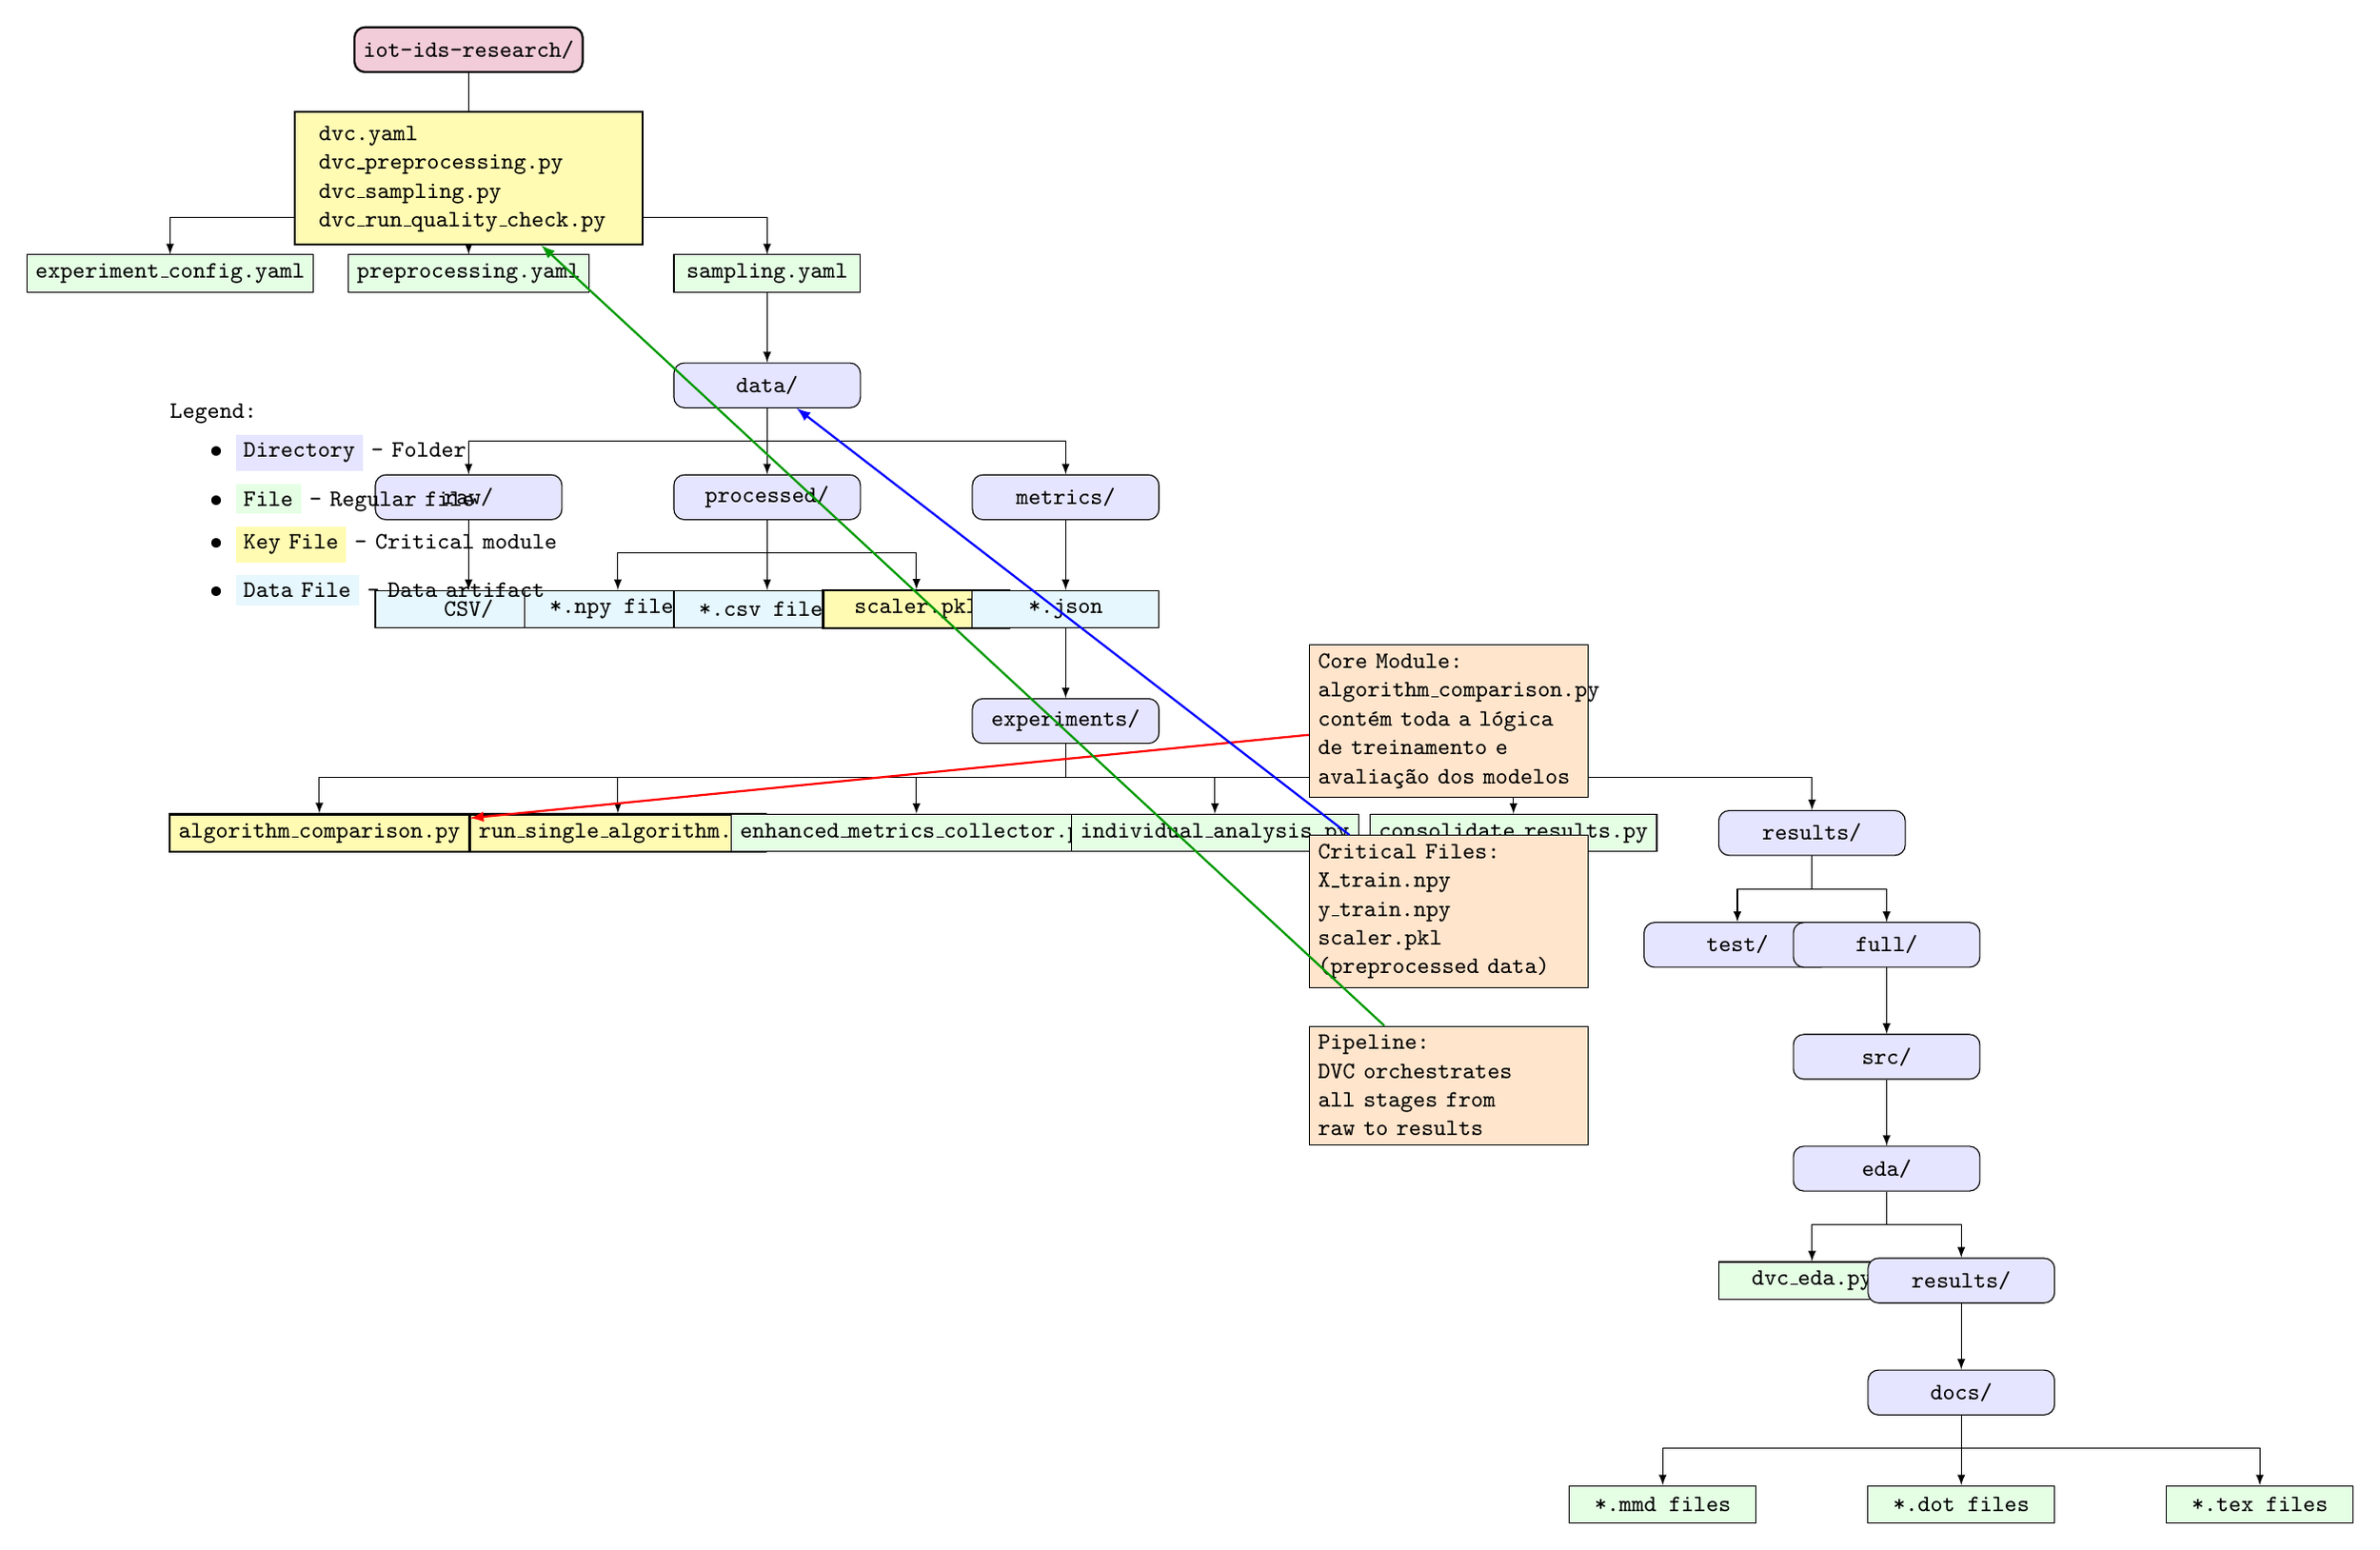
\begin{tikzpicture}[
    % Estilos dos nós
    every node/.style={font=\small\ttfamily},
    dir/.style={draw, rectangle, rounded corners, fill=blue!10, 
                minimum width=2.5cm, minimum height=0.6cm, align=left},
    file/.style={draw, rectangle, fill=green!10, 
                 minimum width=2.5cm, minimum height=0.5cm, align=left},
    key_file/.style={draw, rectangle, fill=yellow!30, 
                     minimum width=2.5cm, minimum height=0.5cm, align=left, thick},
    data_file/.style={draw, rectangle, fill=cyan!10,
                      minimum width=2.5cm, minimum height=0.5cm, align=left},
    level 1/.style={sibling distance=8cm, level distance=1.5cm},
    level 2/.style={sibling distance=4cm, level distance=1.5cm},
    level 3/.style={sibling distance=2cm, level distance=1.5cm},
    edge from parent/.style={draw, -latex}
]

% Root
\node[dir, fill=purple!20, thick] (root) {iot-ids-research/}
    [edge from parent fork down]
    
    % Nível 1 - Principais diretórios
    child { node[dir] (configs) {configs/}
        child { node[file] {experiment\_config.yaml} }
        child { node[file] {preprocessing.yaml} }
        child { node[file] {sampling.yaml} }
    }
    
    child { node[dir] (data) {data/}
        child { node[dir] {raw/}
            child { node[data_file] {CSV/} }
        }
        child { node[dir] {processed/}
            child { node[data_file] {*.npy files} }
            child { node[data_file] {*.csv files} }
            child { node[key_file] {scaler.pkl} }
        }
        child { node[dir] {metrics/}
            child { node[data_file] {*.json} }
        }
    }
    
    child { node[dir] (experiments) {experiments/}
        child { node[key_file] (algo_comp) {algorithm\_comparison.py} }
        child { node[key_file] {run\_single\_algorithm.py} }
        child { node[file] {enhanced\_metrics\_collector.py} }
        child { node[file] {individual\_analysis.py} }
        child { node[file] {consolidate\_results.py} }
        child { node[dir] {results/}
            child { node[dir] {test/} }
            child { node[dir] {full/} }
        }
    }
    
    child { node[dir] (src) {src/}
        child { node[dir] {eda/}
            child { node[file] {dvc\_eda.py} }
            child { node[dir] {results/} }
        }
    }
    
    child { node[dir] (docs) {docs/}
        child { node[file] {*.mmd files} }
        child { node[file] {*.dot files} }
        child { node[file] {*.tex files} }
    };

% DVC scripts no root
\node[key_file, below=0.5cm of root] (dvc_scripts) {
    \begin{tabular}{l}
    dvc.yaml \\
    dvc\_preprocessing.py \\
    dvc\_sampling.py \\
    dvc\_run\_quality\_check.py
    \end{tabular}
};

% Anotações e setas explicativas
\node[draw, rectangle, fill=orange!20, text width=3.5cm, align=left, right=2cm of experiments] (note1) {
    \textbf{Core Module:}\\
    algorithm\_comparison.py\\
    contém toda a lógica\\
    de treinamento e\\
    avaliação dos modelos
};

\draw[-latex, thick, red] (note1) -- (algo_comp);

\node[draw, rectangle, fill=orange!20, text width=3.5cm, align=left, below=0.5cm of note1] (note2) {
    \textbf{Critical Files:}\\
    X\_train.npy\\
    y\_train.npy\\
    scaler.pkl\\
    (preprocessed data)
};

\draw[-latex, thick, blue] (note2) -- (data);

\node[draw, rectangle, fill=orange!20, text width=3.5cm, align=left, below=0.5cm of note2] (note3) {
    \textbf{Pipeline:}\\
    DVC orchestrates\\
    all stages from\\
    raw to results
};

\draw[-latex, thick, green!60!black] (note3) -- (dvc_scripts);

% Legenda
\node[below=2cm of dvc_scripts, text width=8cm, align=left] (legend) {
    \textbf{Legend:}
    \begin{itemize}
        \item \colorbox{blue!10}{Directory} - Folder
        \item \colorbox{green!10}{File} - Regular file
        \item \colorbox{yellow!30}{\textbf{Key File}} - Critical module
        \item \colorbox{cyan!10}{Data File} - Data artifact
    \end{itemize}
};

\end{tikzpicture}

\end{document}

 ou compilar standalone
% ========================================

\documentclass[tikz,border=10pt]{standalone}
\usepackage{tikz}
\usetikzlibrary{trees,positioning,arrows.meta,shapes.geometric,calc}
\usepackage{fontawesome5} % Para ícones (opcional)

\begin{document}

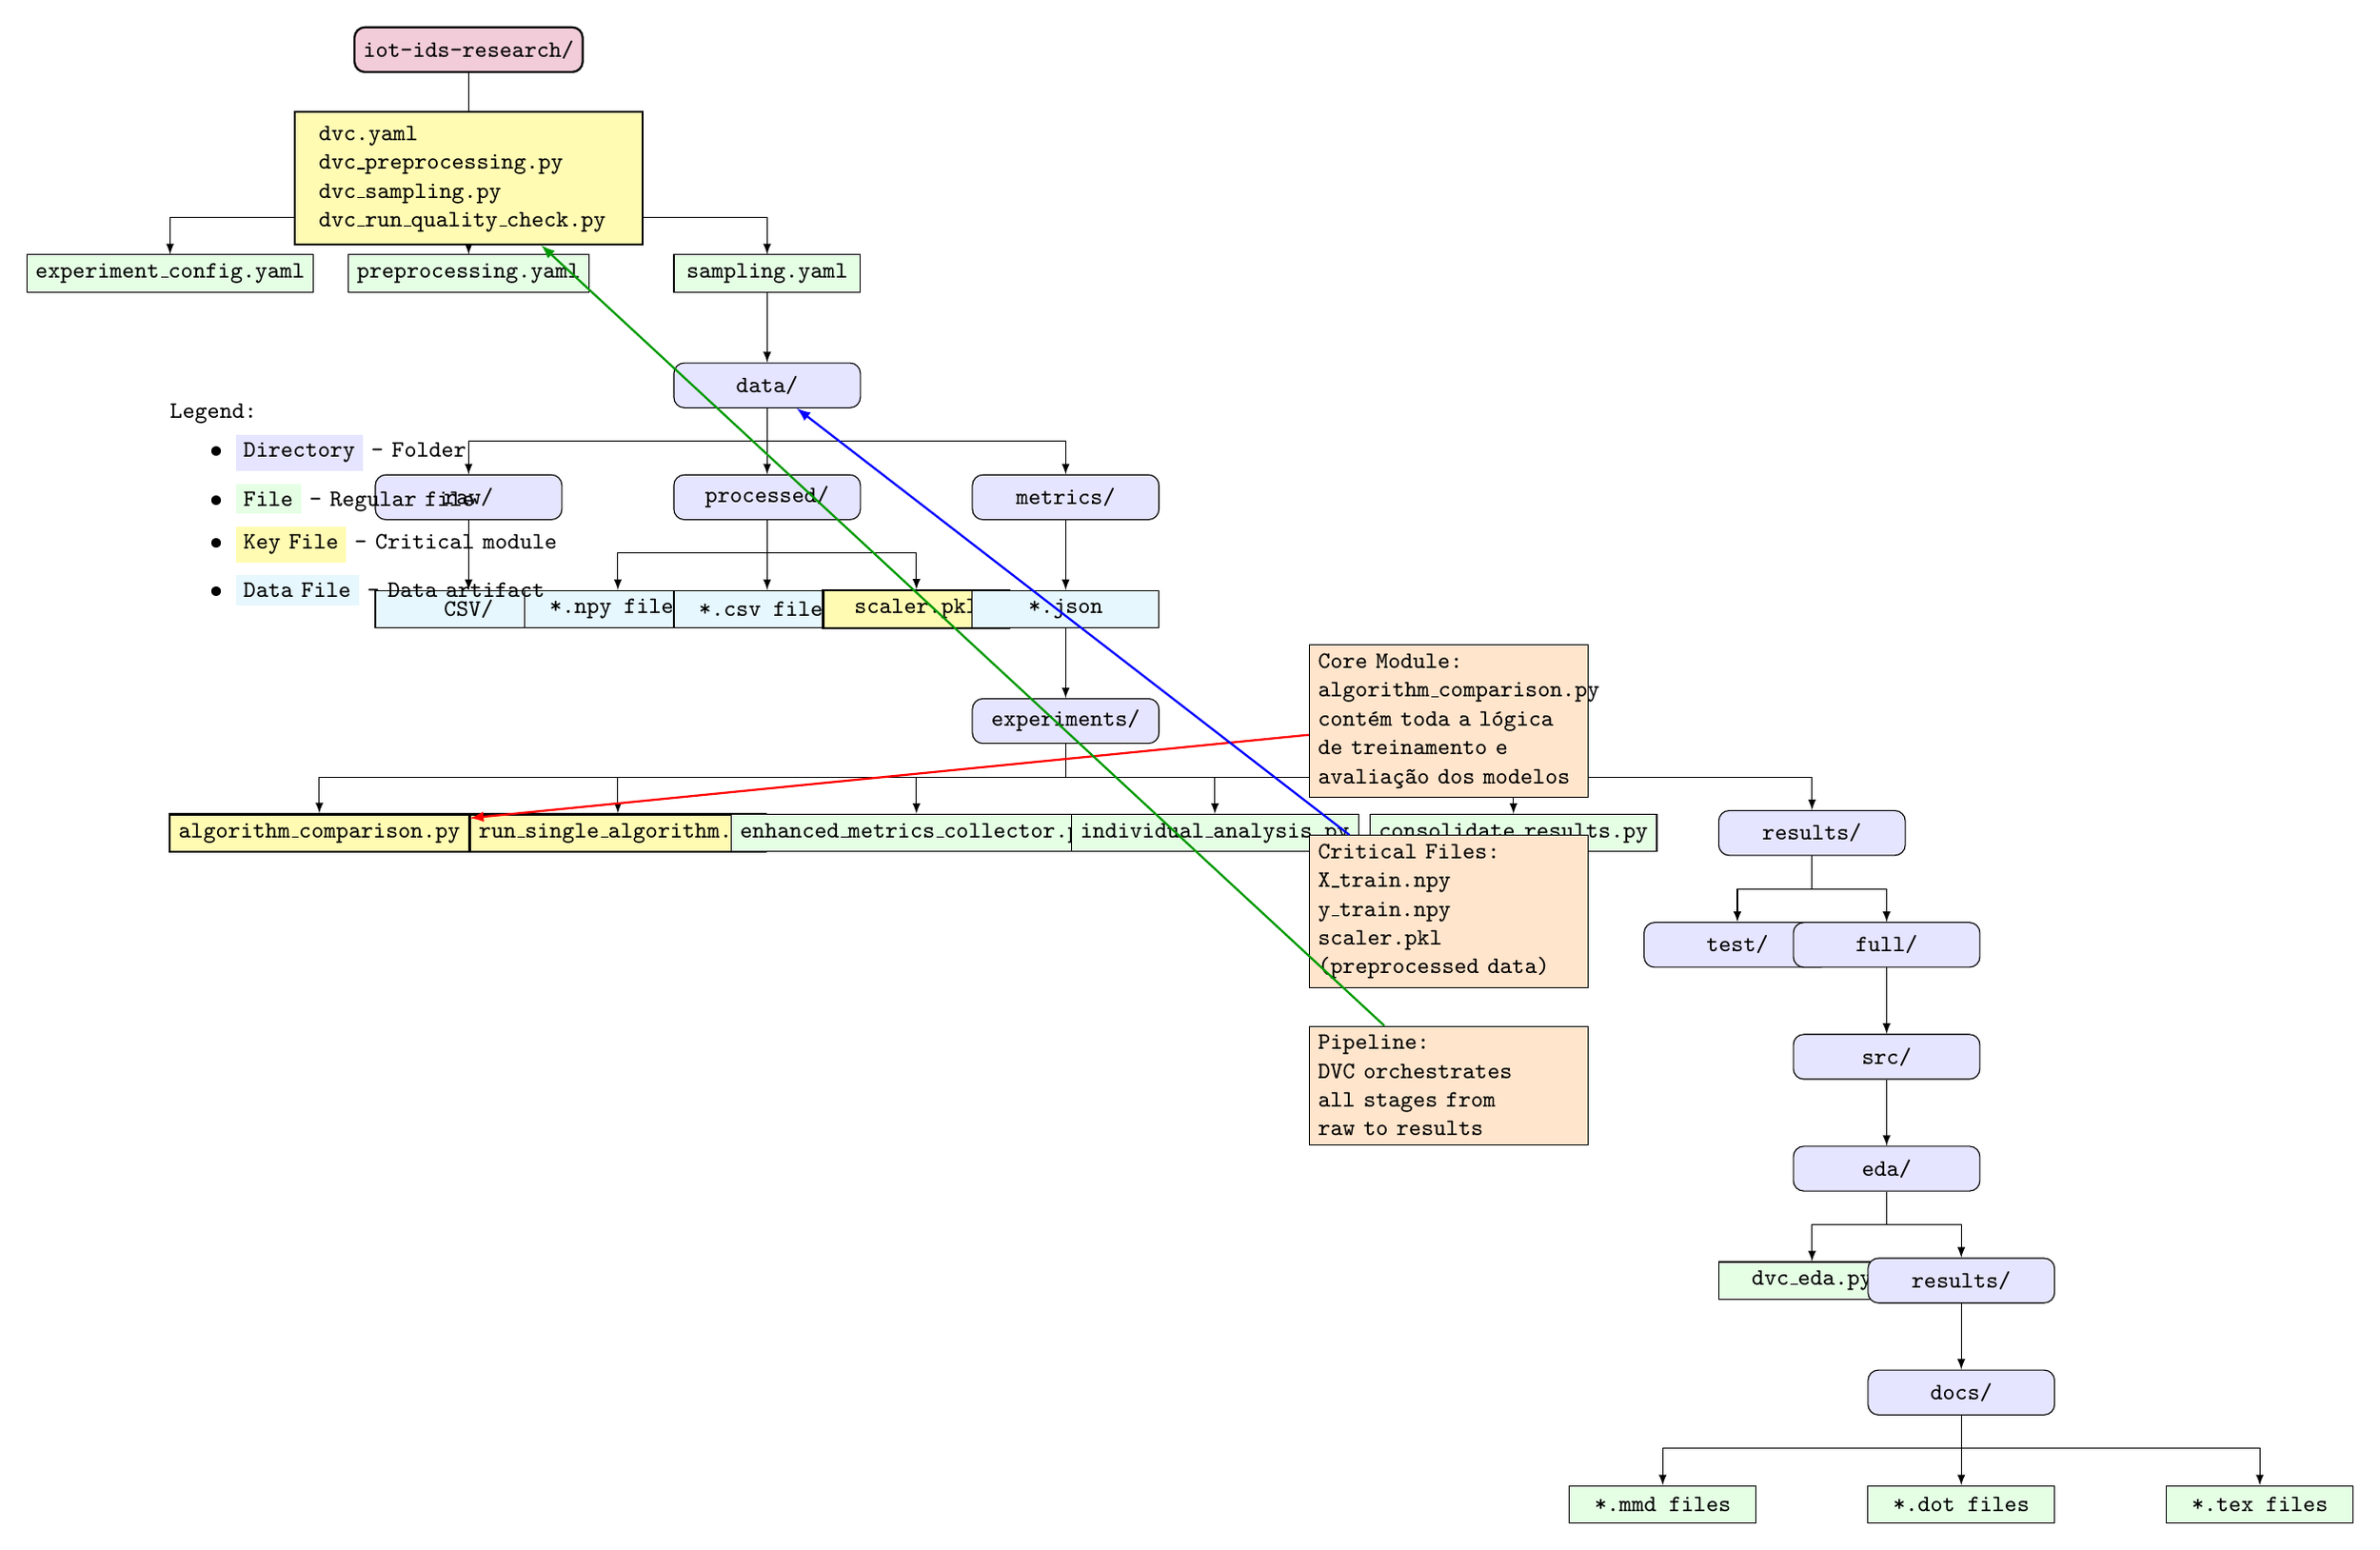
\begin{tikzpicture}[
    % Estilos dos nós
    every node/.style={font=\small\ttfamily},
    dir/.style={draw, rectangle, rounded corners, fill=blue!10, 
                minimum width=2.5cm, minimum height=0.6cm, align=left},
    file/.style={draw, rectangle, fill=green!10, 
                 minimum width=2.5cm, minimum height=0.5cm, align=left},
    key_file/.style={draw, rectangle, fill=yellow!30, 
                     minimum width=2.5cm, minimum height=0.5cm, align=left, thick},
    data_file/.style={draw, rectangle, fill=cyan!10,
                      minimum width=2.5cm, minimum height=0.5cm, align=left},
    level 1/.style={sibling distance=8cm, level distance=1.5cm},
    level 2/.style={sibling distance=4cm, level distance=1.5cm},
    level 3/.style={sibling distance=2cm, level distance=1.5cm},
    edge from parent/.style={draw, -latex}
]

% Root
\node[dir, fill=purple!20, thick] (root) {iot-ids-research/}
    [edge from parent fork down]
    
    % Nível 1 - Principais diretórios
    child { node[dir] (configs) {configs/}
        child { node[file] {experiment\_config.yaml} }
        child { node[file] {preprocessing.yaml} }
        child { node[file] {sampling.yaml} }
    }
    
    child { node[dir] (data) {data/}
        child { node[dir] {raw/}
            child { node[data_file] {CSV/} }
        }
        child { node[dir] {processed/}
            child { node[data_file] {*.npy files} }
            child { node[data_file] {*.csv files} }
            child { node[key_file] {scaler.pkl} }
        }
        child { node[dir] {metrics/}
            child { node[data_file] {*.json} }
        }
    }
    
    child { node[dir] (experiments) {experiments/}
        child { node[key_file] (algo_comp) {algorithm\_comparison.py} }
        child { node[key_file] {run\_single\_algorithm.py} }
        child { node[file] {enhanced\_metrics\_collector.py} }
        child { node[file] {individual\_analysis.py} }
        child { node[file] {consolidate\_results.py} }
        child { node[dir] {results/}
            child { node[dir] {test/} }
            child { node[dir] {full/} }
        }
    }
    
    child { node[dir] (src) {src/}
        child { node[dir] {eda/}
            child { node[file] {dvc\_eda.py} }
            child { node[dir] {results/} }
        }
    }
    
    child { node[dir] (docs) {docs/}
        child { node[file] {*.mmd files} }
        child { node[file] {*.dot files} }
        child { node[file] {*.tex files} }
    };

% DVC scripts no root
\node[key_file, below=0.5cm of root] (dvc_scripts) {
    \begin{tabular}{l}
    dvc.yaml \\
    dvc\_preprocessing.py \\
    dvc\_sampling.py \\
    dvc\_run\_quality\_check.py
    \end{tabular}
};

% Anotações e setas explicativas
\node[draw, rectangle, fill=orange!20, text width=3.5cm, align=left, right=2cm of experiments] (note1) {
    \textbf{Core Module:}\\
    algorithm\_comparison.py\\
    contém toda a lógica\\
    de treinamento e\\
    avaliação dos modelos
};

\draw[-latex, thick, red] (note1) -- (algo_comp);

\node[draw, rectangle, fill=orange!20, text width=3.5cm, align=left, below=0.5cm of note1] (note2) {
    \textbf{Critical Files:}\\
    X\_train.npy\\
    y\_train.npy\\
    scaler.pkl\\
    (preprocessed data)
};

\draw[-latex, thick, blue] (note2) -- (data);

\node[draw, rectangle, fill=orange!20, text width=3.5cm, align=left, below=0.5cm of note2] (note3) {
    \textbf{Pipeline:}\\
    DVC orchestrates\\
    all stages from\\
    raw to results
};

\draw[-latex, thick, green!60!black] (note3) -- (dvc_scripts);

% Legenda
\node[below=2cm of dvc_scripts, text width=8cm, align=left] (legend) {
    \textbf{Legend:}
    \begin{itemize}
        \item \colorbox{blue!10}{Directory} - Folder
        \item \colorbox{green!10}{File} - Regular file
        \item \colorbox{yellow!30}{\textbf{Key File}} - Critical module
        \item \colorbox{cyan!10}{Data File} - Data artifact
    \end{itemize}
};

\end{tikzpicture}

\end{document}

